\documentclass[1p]{elsarticle_modified}
%\bibliographystyle{elsarticle-num}

%\usepackage[colorlinks]{hyperref}
%\usepackage{abbrmath_seonhwa} %\Abb, \Ascr, \Acal ,\Abf, \Afrak
\usepackage{amsfonts}
\usepackage{amssymb}
\usepackage{amsmath}
\usepackage{amsthm}
\usepackage{scalefnt}
\usepackage{amsbsy}
\usepackage{kotex}
\usepackage{caption}
\usepackage{subfig}
\usepackage{color}
\usepackage{graphicx}
\usepackage{xcolor} %% white, black, red, green, blue, cyan, magenta, yellow
\usepackage{float}
\usepackage{setspace}
\usepackage{hyperref}

\usepackage{tikz}
\usetikzlibrary{arrows}

\usepackage{multirow}
\usepackage{array} % fixed length table
\usepackage{hhline}

%%%%%%%%%%%%%%%%%%%%%
\makeatletter
\renewcommand*\env@matrix[1][\arraystretch]{%
	\edef\arraystretch{#1}%
	\hskip -\arraycolsep
	\let\@ifnextchar\new@ifnextchar
	\array{*\c@MaxMatrixCols c}}
\makeatother %https://tex.stackexchange.com/questions/14071/how-can-i-increase-the-line-spacing-in-a-matrix
%%%%%%%%%%%%%%%

\usepackage[normalem]{ulem}

\newcommand{\msout}[1]{\ifmmode\text{\sout{\ensuremath{#1}}}\else\sout{#1}\fi}
%SOURCE: \msout is \stkout macro in https://tex.stackexchange.com/questions/20609/strikeout-in-math-mode

\newcommand{\cancel}[1]{
	\ifmmode
	{\color{red}\msout{#1}}
	\else
	{\color{red}\sout{#1}}
	\fi
}

\newcommand{\add}[1]{
	{\color{blue}\uwave{#1}}
}

\newcommand{\replace}[2]{
	\ifmmode
	{\color{red}\msout{#1}}{\color{blue}\uwave{#2}}
	\else
	{\color{red}\sout{#1}}{\color{blue}\uwave{#2}}
	\fi
}

\newcommand{\Sol}{\mathcal{S}} %segment
\newcommand{\D}{D} %diagram
\newcommand{\A}{\mathcal{A}} %arc


%%%%%%%%%%%%%%%%%%%%%%%%%%%%%5 test

\def\sl{\operatorname{\textup{SL}}(2,\Cbb)}
\def\psl{\operatorname{\textup{PSL}}(2,\Cbb)}
\def\quan{\mkern 1mu \triangleright \mkern 1mu}

\theoremstyle{definition}
\newtheorem{thm}{Theorem}[section]
\newtheorem{prop}[thm]{Proposition}
\newtheorem{lem}[thm]{Lemma}
\newtheorem{ques}[thm]{Question}
\newtheorem{cor}[thm]{Corollary}
\newtheorem{defn}[thm]{Definition}
\newtheorem{exam}[thm]{Example}
\newtheorem{rmk}[thm]{Remark}
\newtheorem{alg}[thm]{Algorithm}

\newcommand{\I}{\sqrt{-1}}
\begin{document}

%\begin{frontmatter}
%
%\title{Boundary parabolic representations of knots up to 8 crossings}
%
%%% Group authors per affiliation:
%\author{Yunhi Cho} 
%\address{Department of Mathematics, University of Seoul, Seoul, Korea}
%\ead{yhcho@uos.ac.kr}
%
%
%\author{Seonhwa Kim} %\fnref{s_kim}}
%\address{Center for Geometry and Physics, Institute for Basic Science, Pohang, 37673, Korea}
%\ead{ryeona17@ibs.re.kr}
%
%\author{Hyuk Kim}
%\address{Department of Mathematical Sciences, Seoul National University, Seoul 08826, Korea}
%\ead{hyukkim@snu.ac.kr}
%
%\author{Seokbeom Yoon}
%\address{Department of Mathematical Sciences, Seoul National University, Seoul, 08826,  Korea}
%\ead{sbyoon15@snu.ac.kr}
%
%\begin{abstract}
%We find all boundary parabolic representation of knots up to 8 crossings.
%
%\end{abstract}
%\begin{keyword}
%    \MSC[2010] 57M25 
%\end{keyword}
%
%\end{frontmatter}

%\linenumbers
%\tableofcontents
%
\newcommand\colored[1]{\textcolor{white}{\rule[-0.35ex]{0.8em}{1.4ex}}\kern-0.8em\color{red} #1}%
%\newcommand\colored[1]{\textcolor{white}{ #1}\kern-2.17ex	\textcolor{white}{ #1}\kern-1.81ex	\textcolor{white}{ #1}\kern-2.15ex\color{red}#1	}

{\Large $\underline{11a_{225}~(K11a_{225})}$}

\setlength{\tabcolsep}{10pt}
\renewcommand{\arraystretch}{1.6}
\vspace{1cm}\begin{tabular}{m{100pt}>{\centering\arraybackslash}m{274pt}}
\multirow{5}{120pt}{
	\centering
	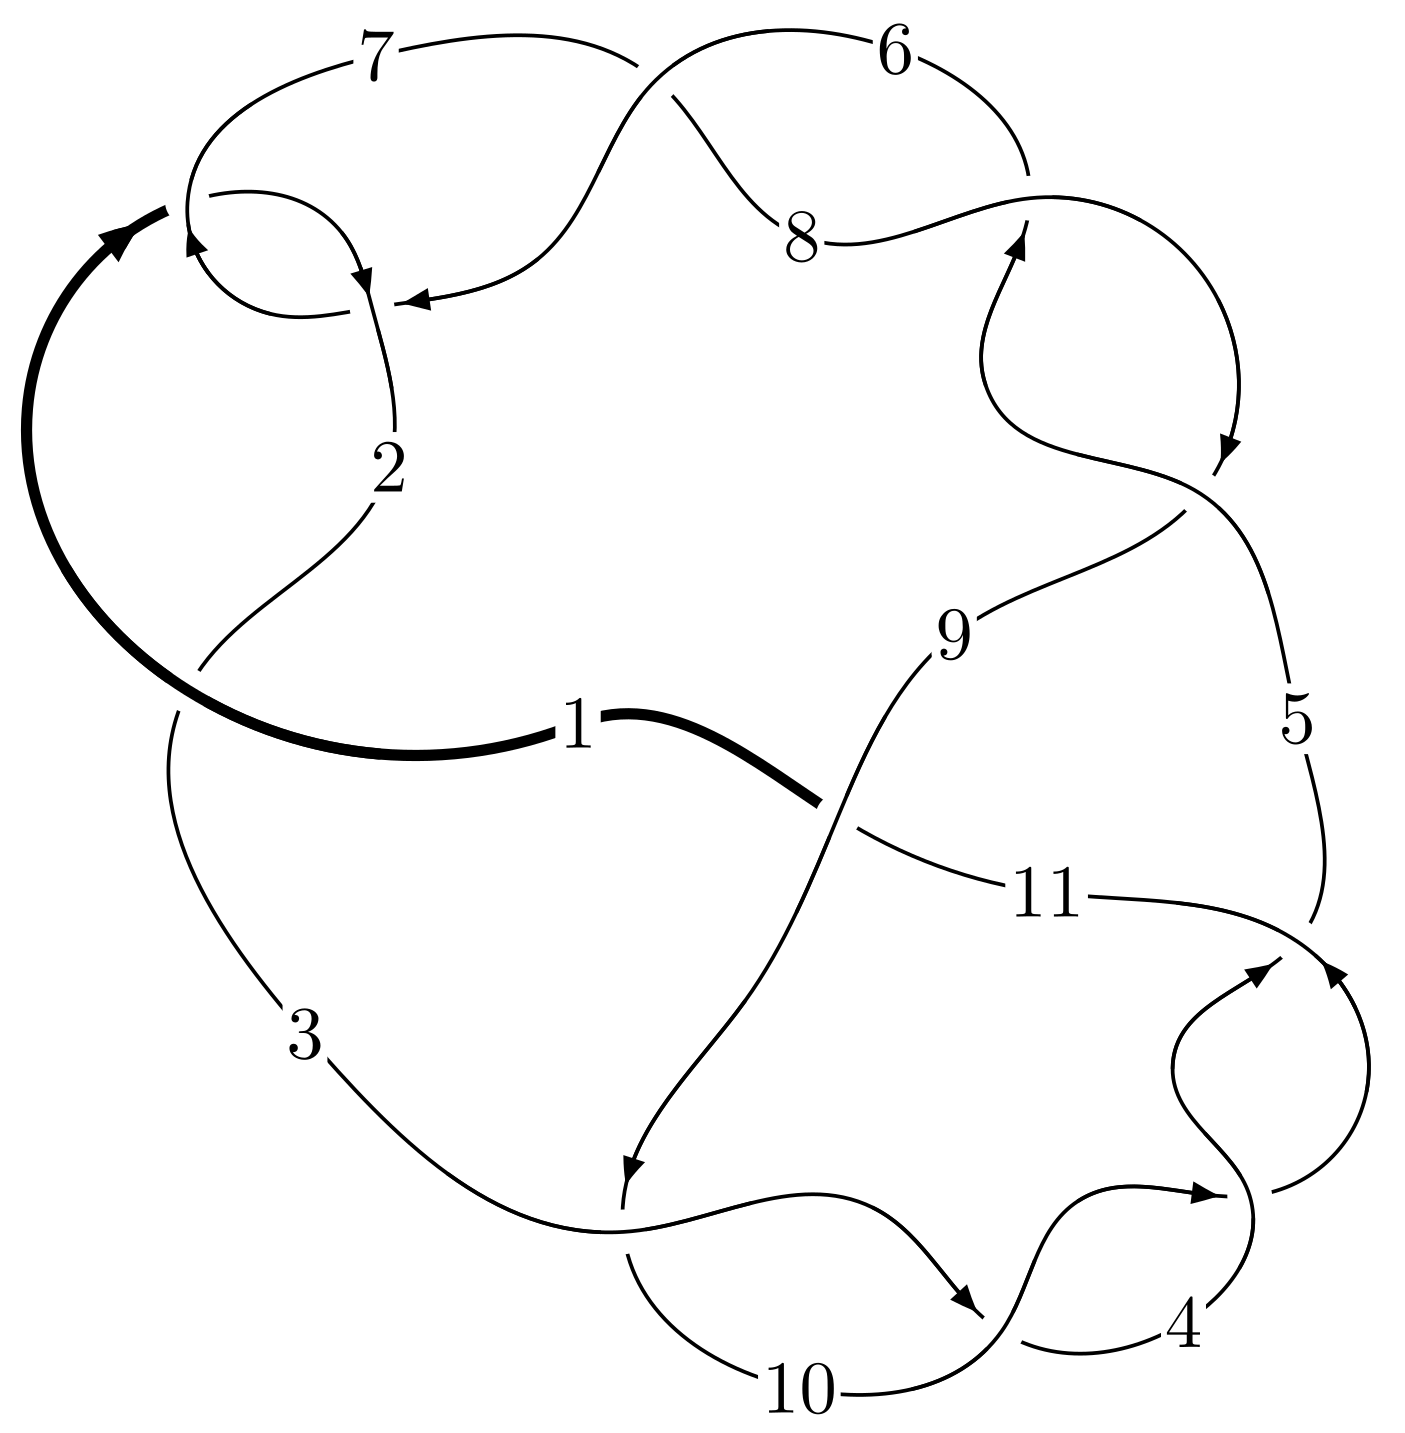
\includegraphics[width=112pt]{../../../GIT/diagram.site/Diagrams/png/474_11a_225.png}\\
\ \ \ A knot diagram\footnotemark}&
\allowdisplaybreaks
\textbf{Linearized knot diagam} \\
\cline{2-2}
 &
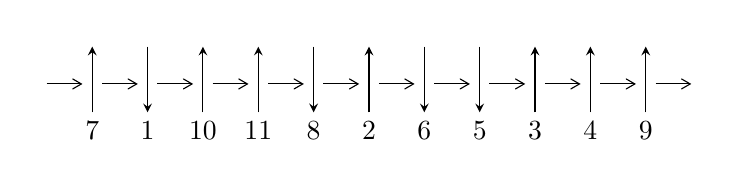
\begin{tikzpicture}[x=20pt, y=17pt]
	% nodes
	\node (C0) at (0, 0) {};
	\node (C1) at (1, 0) {};
	\node (C1U) at (1, +1) {};
	\node (C1D) at (1, -1) {7};

	\node (C2) at (2, 0) {};
	\node (C2U) at (2, +1) {};
	\node (C2D) at (2, -1) {1};

	\node (C3) at (3, 0) {};
	\node (C3U) at (3, +1) {};
	\node (C3D) at (3, -1) {10};

	\node (C4) at (4, 0) {};
	\node (C4U) at (4, +1) {};
	\node (C4D) at (4, -1) {11};

	\node (C5) at (5, 0) {};
	\node (C5U) at (5, +1) {};
	\node (C5D) at (5, -1) {8};

	\node (C6) at (6, 0) {};
	\node (C6U) at (6, +1) {};
	\node (C6D) at (6, -1) {2};

	\node (C7) at (7, 0) {};
	\node (C7U) at (7, +1) {};
	\node (C7D) at (7, -1) {6};

	\node (C8) at (8, 0) {};
	\node (C8U) at (8, +1) {};
	\node (C8D) at (8, -1) {5};

	\node (C9) at (9, 0) {};
	\node (C9U) at (9, +1) {};
	\node (C9D) at (9, -1) {3};

	\node (C10) at (10, 0) {};
	\node (C10U) at (10, +1) {};
	\node (C10D) at (10, -1) {4};

	\node (C11) at (11, 0) {};
	\node (C11U) at (11, +1) {};
	\node (C11D) at (11, -1) {9};
	\node (C12) at (12, 0) {};

	% arrows
	\draw[->,>={angle 60}]
	(C0) edge (C1) (C1) edge (C2) (C2) edge (C3) (C3) edge (C4) (C4) edge (C5) (C5) edge (C6) (C6) edge (C7) (C7) edge (C8) (C8) edge (C9) (C9) edge (C10) (C10) edge (C11) (C11) edge (C12) ;	\draw[->,>=stealth]
	(C1D) edge (C1U) (C2U) edge (C2D) (C3D) edge (C3U) (C4D) edge (C4U) (C5U) edge (C5D) (C6D) edge (C6U) (C7U) edge (C7D) (C8U) edge (C8D) (C9D) edge (C9U) (C10D) edge (C10U) (C11D) edge (C11U) ;
	\end{tikzpicture} \\
\hhline{~~} \\& 
\textbf{Solving Sequence} \\ \cline{2-2} 
 &
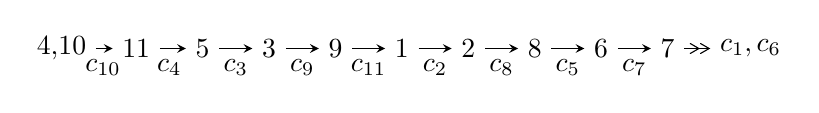
\begin{tikzpicture}[x=24pt, y=7pt]
	% node
	\node (A0) at (-1/8, 0) {4,10};
	\node (A1) at (1, 0) {11};
	\node (A2) at (2, 0) {5};
	\node (A3) at (3, 0) {3};
	\node (A4) at (4, 0) {9};
	\node (A5) at (5, 0) {1};
	\node (A6) at (6, 0) {2};
	\node (A7) at (7, 0) {8};
	\node (A8) at (8, 0) {6};
	\node (A9) at (9, 0) {7};
	\node (C1) at (1/2, -1) {$c_{10}$};
	\node (C2) at (3/2, -1) {$c_{4}$};
	\node (C3) at (5/2, -1) {$c_{3}$};
	\node (C4) at (7/2, -1) {$c_{9}$};
	\node (C5) at (9/2, -1) {$c_{11}$};
	\node (C6) at (11/2, -1) {$c_{2}$};
	\node (C7) at (13/2, -1) {$c_{8}$};
	\node (C8) at (15/2, -1) {$c_{5}$};
	\node (C9) at (17/2, -1) {$c_{7}$};
	\node (A10) at (41/4, 0) {$c_{1},c_{6}$};

	% edge
	\draw[->,>=stealth]	
	(A0) edge (A1) (A1) edge (A2) (A2) edge (A3) (A3) edge (A4) (A4) edge (A5) (A5) edge (A6) (A6) edge (A7) (A7) edge (A8) (A8) edge (A9) ;
	\draw[->>,>={angle 60}]	
	(A9) edge (A10);
\end{tikzpicture} \\ 

\end{tabular} \\

\footnotetext{
The image of knot diagram is generated by the software ``\textbf{Draw programme}" developed by Andrew Bartholomew(\url{http://www.layer8.co.uk/maths/draw/index.htm\#Running-draw}), where we modified some parts for our purpose(\url{https://github.com/CATsTAILs/LinksPainter}).
}\phantom \\ \newline 
\centering \textbf{Ideals for irreducible components\footnotemark of $X_{\text{par}}$} 
 
\begin{align*}
I^u_{1}&=\langle 
u^{26}- u^{25}+\cdots- u-1\rangle \\
\\
\end{align*}
\raggedright * 1 irreducible components of $\dim_{\mathbb{C}}=0$, with total 26 representations.\\
\footnotetext{All coefficients of polynomials are rational numbers. But the coefficients are sometimes approximated in decimal forms when there is not enough margin.}
\newpage
\renewcommand{\arraystretch}{1}
\centering \section*{I. $I^u_{1}= \langle u^{26}- u^{25}+\cdots- u-1 \rangle$}
\flushleft \textbf{(i) Arc colorings}\\
\begin{tabular}{m{7pt} m{180pt} m{7pt} m{180pt} }
\flushright $a_{4}=$&$\begin{pmatrix}0\\u\end{pmatrix}$ \\
\flushright $a_{10}=$&$\begin{pmatrix}1\\0\end{pmatrix}$ \\
\flushright $a_{11}=$&$\begin{pmatrix}1\\- u^2\end{pmatrix}$ \\
\flushright $a_{5}=$&$\begin{pmatrix}u\\- u^3+u\end{pmatrix}$ \\
\flushright $a_{3}=$&$\begin{pmatrix}- u\\u\end{pmatrix}$ \\
\flushright $a_{9}=$&$\begin{pmatrix}- u^2+1\\u^2\end{pmatrix}$ \\
\flushright $a_{1}=$&$\begin{pmatrix}- u^6+3 u^4-2 u^2+1\\u^6-2 u^4- u^2\end{pmatrix}$ \\
\flushright $a_{2}=$&$\begin{pmatrix}- u^{11}+6 u^9-12 u^7+10 u^5-5 u^3\\u^{11}-5 u^9+6 u^7+u^5- u^3+u\end{pmatrix}$ \\
\flushright $a_{8}=$&$\begin{pmatrix}- u^6+3 u^4-2 u^2+1\\u^8-4 u^6+4 u^4\end{pmatrix}$ \\
\flushright $a_{6}=$&$\begin{pmatrix}u^{11}-6 u^9+12 u^7-10 u^5+5 u^3\\- u^{13}+7 u^{11}-17 u^9+16 u^7-4 u^5- u^3+u\end{pmatrix}$ \\
\flushright $a_{7}=$&$\begin{pmatrix}- u^{16}+9 u^{14}-31 u^{12}+52 u^{10}-47 u^8+24 u^6-2 u^4-2 u^2+1\\u^{18}-10 u^{16}+39 u^{14}-74 u^{12}+69 u^{10}-26 u^8-4 u^6+8 u^4- u^2\end{pmatrix}$\\ \flushright $a_{7}=$&$\begin{pmatrix}- u^{16}+9 u^{14}-31 u^{12}+52 u^{10}-47 u^8+24 u^6-2 u^4-2 u^2+1\\u^{18}-10 u^{16}+39 u^{14}-74 u^{12}+69 u^{10}-26 u^8-4 u^6+8 u^4- u^2\end{pmatrix}$\\&\end{tabular}
\flushleft \textbf{(ii) Obstruction class $= -1$}\\~\\
\flushleft \textbf{(iii) Cusp Shapes $= -4 u^{23}+56 u^{21}-328 u^{19}-4 u^{18}+1040 u^{17}+44 u^{16}-1936 u^{15}-192 u^{14}+2156 u^{13}+420 u^{12}-1376 u^{11}-484 u^{10}+324 u^9+288 u^8+228 u^7-60 u^6-176 u^5-52 u^4+52 u^3+20 u^2+12 u+2$}\\~\\
\newpage\renewcommand{\arraystretch}{1}
\flushleft \textbf{(iv) u-Polynomials at the component}\newline \\
\begin{tabular}{m{50pt}|m{274pt}}
Crossings & \hspace{64pt}u-Polynomials at each crossing \\
\hline $$\begin{aligned}c_{1},c_{6}\end{aligned}$$&$\begin{aligned}
&u^{26}+u^{25}+\cdots+u-1
\end{aligned}$\\
\hline $$\begin{aligned}c_{2},c_{5},c_{7}\\c_{8}\end{aligned}$$&$\begin{aligned}
&u^{26}+5 u^{25}+\cdots-3 u+1
\end{aligned}$\\
\hline $$\begin{aligned}c_{3},c_{4},c_{9}\\c_{10}\end{aligned}$$&$\begin{aligned}
&u^{26}- u^{25}+\cdots- u-1
\end{aligned}$\\
\hline $$\begin{aligned}c_{11}\end{aligned}$$&$\begin{aligned}
&u^{26}+9 u^{25}+\cdots-247 u-89
\end{aligned}$\\
\hline
\end{tabular}\\~\\
\newpage\renewcommand{\arraystretch}{1}
\flushleft \textbf{(v) Riley Polynomials at the component}\newline \\
\begin{tabular}{m{50pt}|m{274pt}}
Crossings & \hspace{64pt}Riley Polynomials at each crossing \\
\hline $$\begin{aligned}c_{1},c_{6}\end{aligned}$$&$\begin{aligned}
&y^{26}+5 y^{25}+\cdots-3 y+1
\end{aligned}$\\
\hline $$\begin{aligned}c_{2},c_{5},c_{7}\\c_{8}\end{aligned}$$&$\begin{aligned}
&y^{26}+33 y^{25}+\cdots-59 y+1
\end{aligned}$\\
\hline $$\begin{aligned}c_{3},c_{4},c_{9}\\c_{10}\end{aligned}$$&$\begin{aligned}
&y^{26}-31 y^{25}+\cdots-3 y+1
\end{aligned}$\\
\hline $$\begin{aligned}c_{11}\end{aligned}$$&$\begin{aligned}
&y^{26}-19 y^{25}+\cdots-92159 y+7921
\end{aligned}$\\
\hline
\end{tabular}\\~\\
\newpage\flushleft \textbf{(vi) Complex Volumes and Cusp Shapes}
$$\begin{array}{c|c|c}  
\text{Solutions to }I^u_{1}& \I (\text{vol} + \sqrt{-1}CS) & \text{Cusp shape}\\
 \hline 
\begin{aligned}
u &= \phantom{-}0.839779 + 0.452868 I\end{aligned}
 & \phantom{-}11.16140 + 0.44023 I & \phantom{-}10.10436 - 1.46145 I \\ \hline\begin{aligned}
u &= \phantom{-}0.839779 - 0.452868 I\end{aligned}
 & \phantom{-}11.16140 - 0.44023 I & \phantom{-}10.10436 + 1.46145 I \\ \hline\begin{aligned}
u &= -0.825387 + 0.468991 I\end{aligned}
 & \phantom{-}11.03030 - 7.05835 I & \phantom{-}9.75996 + 6.21969 I \\ \hline\begin{aligned}
u &= -0.825387 - 0.468991 I\end{aligned}
 & \phantom{-}11.03030 + 7.05835 I & \phantom{-}9.75996 - 6.21969 I \\ \hline\begin{aligned}
u &= -0.684207 + 0.398529 I\end{aligned}
 & \phantom{-}1.89109 - 4.88723 I & \phantom{-}7.24553 + 8.84366 I \\ \hline\begin{aligned}
u &= -0.684207 - 0.398529 I\end{aligned}
 & \phantom{-}1.89109 + 4.88723 I & \phantom{-}7.24553 - 8.84366 I \\ \hline\begin{aligned}
u &= \phantom{-}0.733274 + 0.287832 I\end{aligned}
 & \phantom{-}2.67984 + 0.49611 I & \phantom{-}10.71301 - 1.37639 I \\ \hline\begin{aligned}
u &= \phantom{-}0.733274 - 0.287832 I\end{aligned}
 & \phantom{-}2.67984 - 0.49611 I & \phantom{-}10.71301 + 1.37639 I \\ \hline\begin{aligned}
u &= -0.012357 + 0.660147 I\end{aligned}
 & \phantom{-}8.58736 + 3.27967 I & \phantom{-}5.99252 - 2.35106 I \\ \hline\begin{aligned}
u &= -0.012357 - 0.660147 I\end{aligned}
 & \phantom{-}8.58736 - 3.27967 I & \phantom{-}5.99252 + 2.35106 I \\ \hline\begin{aligned}
u &= -0.439187 + 0.350365 I\end{aligned}
 & -1.41635 - 1.31903 I & -1.30126 + 6.10882 I \\ \hline\begin{aligned}
u &= -0.439187 - 0.350365 I\end{aligned}
 & -1.41635 + 1.31903 I & -1.30126 - 6.10882 I \\ \hline\begin{aligned}
u &= \phantom{-}0.525085\phantom{ +0.000000I}\end{aligned}
 & \phantom{-}0.783407\phantom{ +0.000000I} & \phantom{-}12.8960\phantom{ +0.000000I} \\ \hline\begin{aligned}
u &= -0.106020 + 0.464476 I\end{aligned}
 & \phantom{-}0.26125 + 1.87689 I & \phantom{-}2.74450 - 3.73316 I \\ \hline\begin{aligned}
u &= -0.106020 - 0.464476 I\end{aligned}
 & \phantom{-}0.26125 - 1.87689 I & \phantom{-}2.74450 + 3.73316 I \\ \hline\begin{aligned}
u &= \phantom{-}1.54395 + 0.04489 I\end{aligned}
 & \phantom{-}5.28037 + 2.44629 I & \phantom{-}3.67676 - 4.11819 I \\ \hline\begin{aligned}
u &= \phantom{-}1.54395 - 0.04489 I\end{aligned}
 & \phantom{-}5.28037 - 2.44629 I & \phantom{-}3.67676 + 4.11819 I \\ \hline\begin{aligned}
u &= -1.58507\phantom{ +0.000000I}\end{aligned}
 & \phantom{-}8.17274\phantom{ +0.000000I} & \phantom{-}12.1060\phantom{ +0.000000I} \\ \hline\begin{aligned}
u &= \phantom{-}1.59973 + 0.10370 I\end{aligned}
 & \phantom{-}9.67676 + 6.71425 I & \phantom{-}9.25508 - 6.45300 I \\ \hline\begin{aligned}
u &= \phantom{-}1.59973 - 0.10370 I\end{aligned}
 & \phantom{-}9.67676 - 6.71425 I & \phantom{-}9.25508 + 6.45300 I \\ \hline\begin{aligned}
u &= -1.61572 + 0.07479 I\end{aligned}
 & \phantom{-}10.74900 - 1.83401 I & \phantom{-}11.98633 + 0.23070 I \\ \hline\begin{aligned}
u &= -1.61572 - 0.07479 I\end{aligned}
 & \phantom{-}10.74900 + 1.83401 I & \phantom{-}11.98633 - 0.23070 I \\ \hline\begin{aligned}
u &= \phantom{-}1.64863 + 0.13284 I\end{aligned}
 & \phantom{-}19.5205 + 9.3622 I & \phantom{-}11.47654 - 4.95795 I \\ \hline\begin{aligned}
u &= \phantom{-}1.64863 - 0.13284 I\end{aligned}
 & \phantom{-}19.5205 - 9.3622 I & \phantom{-}11.47654 + 4.95795 I \\ \hline\begin{aligned}
u &= -1.65250 + 0.12610 I\end{aligned}
 & \phantom{-}19.7312 - 2.6570 I & \phantom{-}11.84579 + 0.35212 I \\ \hline\begin{aligned}
u &= -1.65250 - 0.12610 I\end{aligned}
 & \phantom{-}19.7312 + 2.6570 I & \phantom{-}11.84579 - 0.35212 I\\
 \hline 
 \end{array}$$\newpage
\newpage\renewcommand{\arraystretch}{1}
\centering \section*{ II. u-Polynomials}
\begin{tabular}{m{50pt}|m{274pt}}
Crossings & \hspace{64pt}u-Polynomials at each crossing \\
\hline $$\begin{aligned}c_{1},c_{6}\end{aligned}$$&$\begin{aligned}
&u^{26}+u^{25}+\cdots+u-1
\end{aligned}$\\
\hline $$\begin{aligned}c_{2},c_{5},c_{7}\\c_{8}\end{aligned}$$&$\begin{aligned}
&u^{26}+5 u^{25}+\cdots-3 u+1
\end{aligned}$\\
\hline $$\begin{aligned}c_{3},c_{4},c_{9}\\c_{10}\end{aligned}$$&$\begin{aligned}
&u^{26}- u^{25}+\cdots- u-1
\end{aligned}$\\
\hline $$\begin{aligned}c_{11}\end{aligned}$$&$\begin{aligned}
&u^{26}+9 u^{25}+\cdots-247 u-89
\end{aligned}$\\
\hline
\end{tabular}\newpage\renewcommand{\arraystretch}{1}
\centering \section*{ III. Riley Polynomials}
\begin{tabular}{m{50pt}|m{274pt}}
Crossings & \hspace{64pt}Riley Polynomials at each crossing \\
\hline $$\begin{aligned}c_{1},c_{6}\end{aligned}$$&$\begin{aligned}
&y^{26}+5 y^{25}+\cdots-3 y+1
\end{aligned}$\\
\hline $$\begin{aligned}c_{2},c_{5},c_{7}\\c_{8}\end{aligned}$$&$\begin{aligned}
&y^{26}+33 y^{25}+\cdots-59 y+1
\end{aligned}$\\
\hline $$\begin{aligned}c_{3},c_{4},c_{9}\\c_{10}\end{aligned}$$&$\begin{aligned}
&y^{26}-31 y^{25}+\cdots-3 y+1
\end{aligned}$\\
\hline $$\begin{aligned}c_{11}\end{aligned}$$&$\begin{aligned}
&y^{26}-19 y^{25}+\cdots-92159 y+7921
\end{aligned}$\\
\hline
\end{tabular}
\vskip 2pc
\end{document}